\documentclass{beamer}
\usepackage[utf8]{inputenc}
\usepackage{graphicx, epsfig}
\usepackage{amsmath,mathrsfs,amsfonts,amssymb}
%\usepackage{subfig}
\usepackage{floatflt}
\usepackage{epic,ecltree}
\usepackage{mathtext}
\usepackage{fancybox}
\usepackage{fancyhdr}
\usepackage{multirow}
\usepackage{enumerate}
\usepackage{epstopdf}
\usepackage{multicol}
\usepackage{algorithm}
\usepackage[noend]{algorithmic}
\def\algorithmicrequire{\textbf{Input:}}
\def\algorithmicensure{\textbf{Output:}}
\usetheme{default}%{Singapore}%{Warsaw}%{Warsaw}%{Darmstadt}
\usecolortheme{default}
\setbeamertemplate{footline}[page number]{}
\setbeamerfont{title}{size=\Huge}


\newcommand{\bh}{\mathbf{h}} 
\newcommand{\bt}{\mathbf{t}} 
\newcommand{\bu}{\mathbf{u}} 
\newcommand{\bv}{\mathbf{v}} 
\newcommand{\bw}{\mathbf{w}} 
\newcommand{\bx}{\mathbf{x}} 
\newcommand{\bz}{\mathbf{z}} 
\newcommand{\by}{\mathbf{y}} 

\newcommand{\bA}{\mathbf{A}} 
\newcommand{\bC}{\mathbf{C}} 
\newcommand{\bI}{\mathbf{I}} 
\newcommand{\bT}{\mathbf{T}} 
\newcommand{\bW}{\mathbf{W}} 
\newcommand{\bX}{\mathbf{X}} 
\newcommand{\bZ}{\mathbf{Z}} 

\newcommand{\bepsilon}{\boldsymbol{\epsilon}}
\newcommand{\bmu}{\boldsymbol{\mu}}
\newcommand{\blambda}{\boldsymbol{\lambda}}
\newcommand{\bsigma}{\boldsymbol{\sigma}}
\newcommand{\bSigma}{\boldsymbol{\Sigma}}

\newcommand{\bbE}{\mathbb{E}} 
\newcommand{\bbP}{\mathbb{P}} 
\newcommand{\bbR}{\mathbb{R}} 

\newcommand{\cL}{\mathcal{L}} 
\newcommand{\cN}{\mathcal{N}} 
\newcommand{\cS}{\mathcal{S}} 
\newcommand{\cT}{\mathcal{T}} 
\newcommand{\cX}{\mathcal{X}} 

\newcommand{\btheta}{\boldsymbol{\theta}} 
\newcommand{\bphi}{\boldsymbol{\phi}} 

\DeclareMathOperator*{\argmin}{arg\,min}
\DeclareMathOperator*{\argmax}{arg\,max}

%\definecolor{beamer@blendedblue}{RGB}{15,120,80}
%----------------------------------------------------------------------------------------------------------
\title[\hbox to 56mm{Deep Generative Models  \hfill\insertframenumber\,/\,\inserttotalframenumber}]
{Deep Generative Models \\ Lecture 10}
\author[Roman Isachenko]{\\Roman Isachenko}
\institute[MIPT]{Moscow Institute of Physics and Technology \\
}
\date{2020}
%--------------------------------------------------------------------------------
\begin{document}
%--------------------------------------------------------------------------------
\begin{frame}
%\thispagestyle{empty}
\titlepage
\end{frame}
%=======
\begin{frame}{Evaluation of likelihood-free models}
	How to evaluate generative models?
	\begin{block}{Likelihood-based models}
		\begin{itemize}
			\item Split data to train/val/test.
			\item Fit model on the train part.
			\item Tune hyperparameters on the validation part.
			\item Evaluate generalization by reporting likelihoods on the test set.
		\end{itemize}
	\end{block}
	\begin{block}{Not all models have tractable likelihoods}
		\begin{itemize}
			\item VAE: compare ELBO values.
			\item GAN: ???
		\end{itemize}
	\end{block}
\end{frame}
%=======
\begin{frame}{Evaluation of likelihood-free models}
	Let take some pretrained image classification model to get the conditional label distribution $p(y | \bx)$ (e.g. ImageNet classifier).
	\begin{block}{What do we want from samples?}
		\begin{itemize}
			\item \textbf{Sharpness}
			\begin{figure}
				\centering
				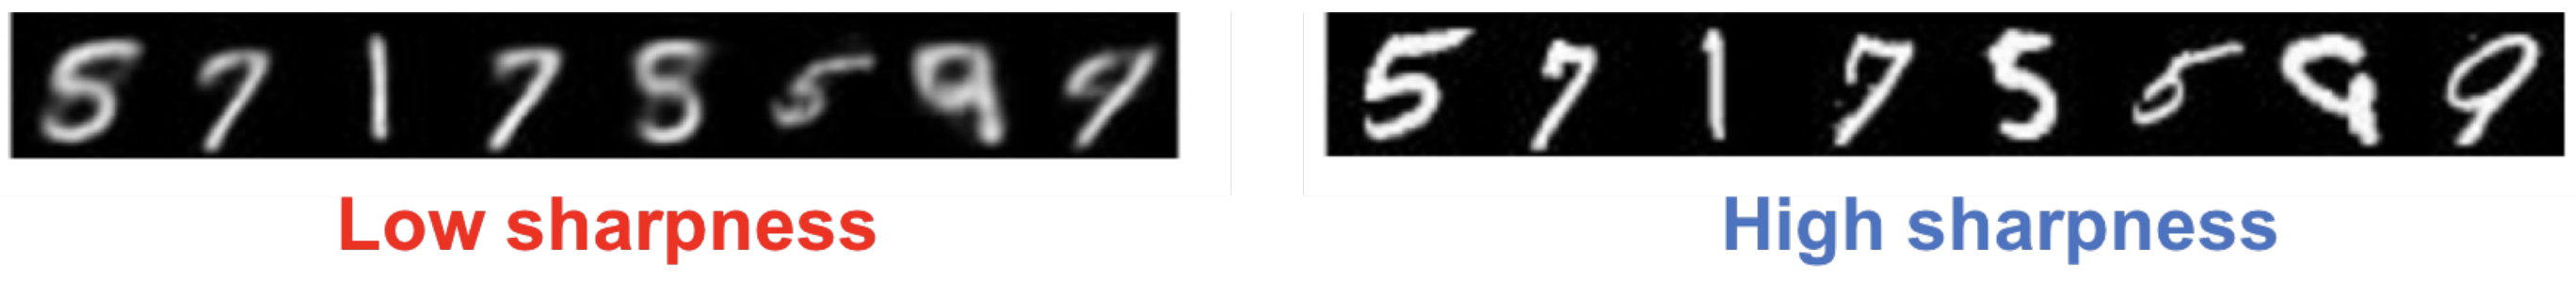
\includegraphics[width=0.9\linewidth]{figs/sharpness}
			\end{figure}
			The conditional distribution $p(y | \bx)$ should have low entropy (each image $\bx$ should have distinctly recognizable object).
			\item \textbf{Diversity}
			\begin{figure}
				\centering
				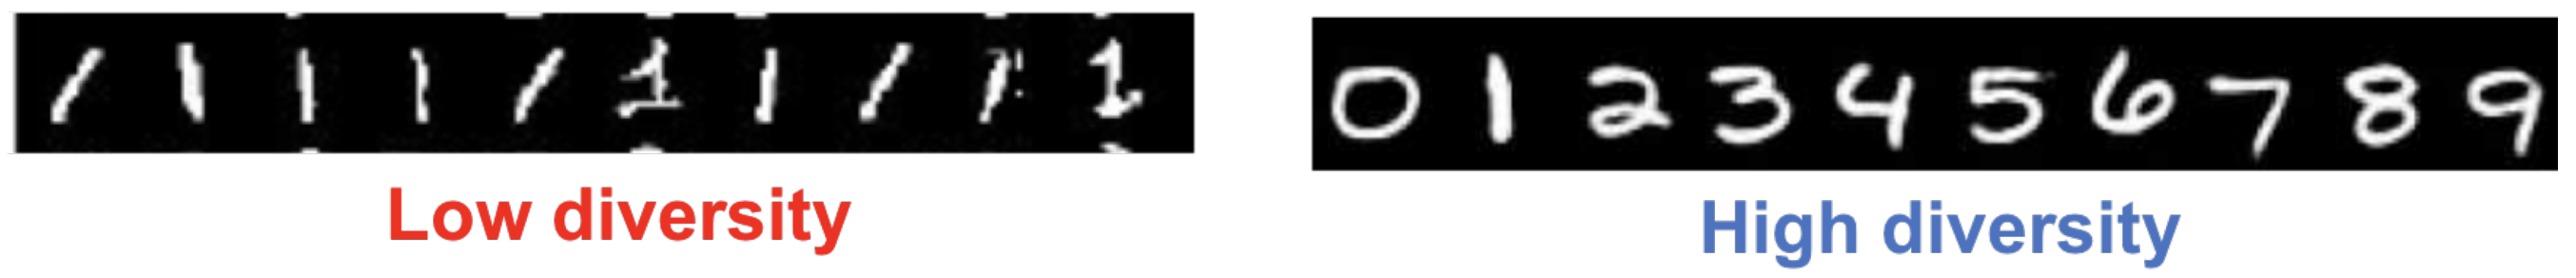
\includegraphics[width=0.9\linewidth]{figs/diversity}
			\end{figure}
			The marginal distribution $p(y) = \int p(y | \bx) p(\bx) d \bx$ should have high entropy (there should be as many classes generated as possible).
		\end{itemize}
	\end{block}
	\vfill
	\hrule\medskip 
	{\scriptsize \href{https://deepgenerativemodels.github.io}{https://deepgenerativemodels.github.io}}
\end{frame}
%=======
\begin{frame}{Evaluation of likelihood-free models}
	\begin{block}{What do we want from samples?}
		\begin{itemize}
			\item \textbf{Sharpness.}
			The conditional distribution $p(y | \bx)$ should have low entropy (each image $\bx$ should have distinctly recognizable object).
			\item \textbf{Diversity.}
			The marginal distribution $p(y) = \int p(y | \bx) p(\bx) d \bx$ should have high entropy (there should be as many classes generated as possible).
		\end{itemize}
	\end{block}
	\begin{figure}
		\centering
		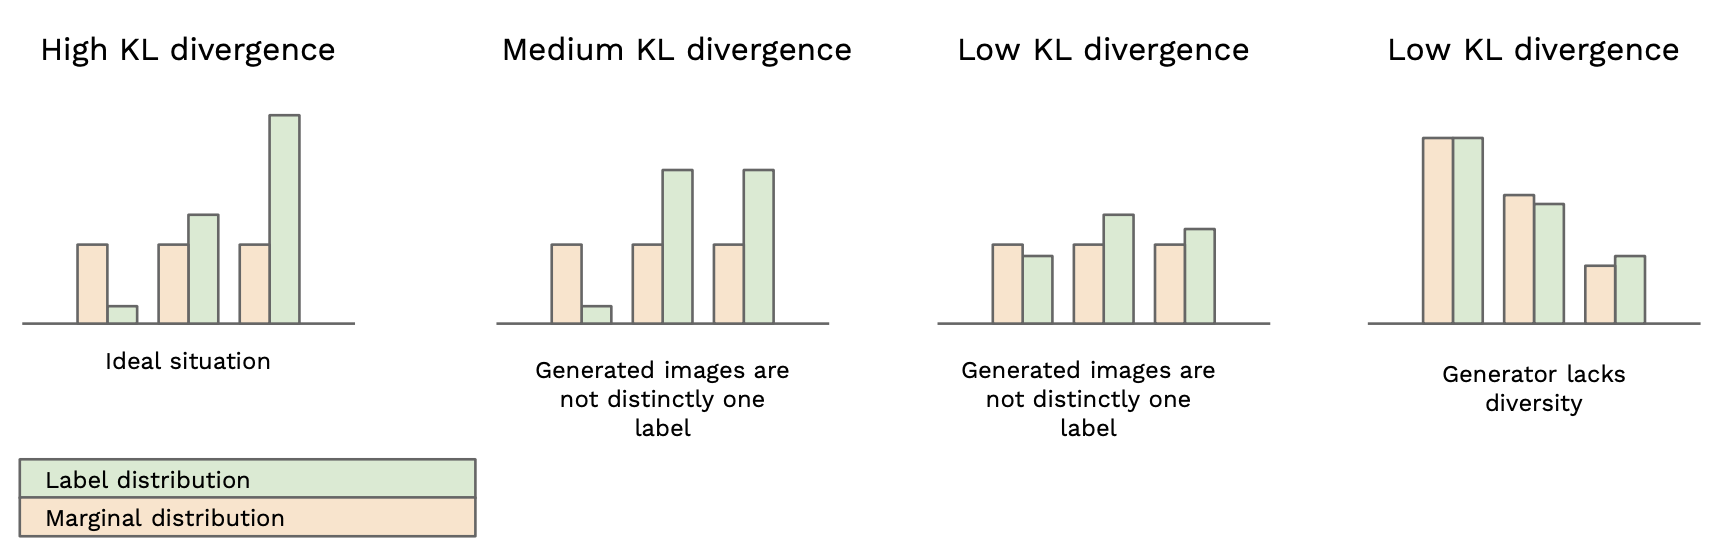
\includegraphics[width=1.0\linewidth]{figs/is_toy}
	\end{figure}
	\vfill
	\hrule\medskip 
	{\scriptsize \href{https://medium.com/octavian-ai/a-simple-explanation-of-the-inception-score-372dff6a8c7a}{https://medium.com/octavian-ai/a-simple-explanation-of-the-inception-score-372dff6a8c7a}}
\end{frame}
%=======
\begin{frame}{Evaluation of likelihood-free models}
		\begin{block}{What do we want from samples?}
		\begin{itemize}
			\item Sharpness $\Rightarrow$ low $H(y | \bx) = - \sum_{y} \int_{\bx} p(y, \bx) \log p(y | \bx) d\bx$.
			\item Diversity $\Rightarrow$ high $H(y)  = - \sum_{y} p(y) \log p(y)$.
		\end{itemize}
	\end{block}
	\begin{block}{Inception Score}
		\vspace{-0.3cm}
		\footnotesize
		\begin{align*}
			IS &= \exp(H(y) - H(y | \bx)) \\ 
			&= \exp \left( - \sum_{y} p(y) \log p(y) + \sum_{y} \int_{\bx} p(y, \bx) \log p(y | \bx) d\bx\right) \\
			&= \exp \left( \sum_{y} \int_{\bx} p(y, \bx) \log \frac{p(y | \bx)}{p(y)} d\bx\right) \\ 
			&= \exp \left( \bbE_{\bx} \sum_{y} p(y | \bx) \log \frac{p(y | \bx)}{p(y)} \right) = \exp \left( \bbE_{\bx} KL(p(y | \bx) || p(y)) \right)
		\end{align*}
	\end{block}
	\vfill
	\hrule\medskip 
	{\scriptsize \href{https://arxiv.org/abs/1606.03498}{https://arxiv.org/abs/1606.03498}}
\end{frame}
%=======
\begin{frame}{Evaluation of likelihood-free models}
	\begin{block}{Inception Score}
		\vspace{-0.1cm}
		\[
			IS =  \exp \left( \bbE_{\bx} KL(p(y | \bx) || p(y)) \right)
		\]
		\vspace{-0.1cm}
	\end{block}
	\begin{block}{IS limitations}
		\begin{itemize}
			\item Inception score depends on the quality of the pretrained classifier $p(y | \bx)$.
			\item If generator produces images with a different set of labels from the classifier training set, IS will be low.
			\item If the generator produces one image per class, the IS will be perfect (there is no measure of intra-class diversity).
			\item IS only require samples from the generator and do not take into account the desired data distribution $\pi(\bx)$ directly (only implicitly via a classifier).
		\end{itemize}
	\end{block}
	\vfill
	\hrule\medskip 
	{\scriptsize \href{https://arxiv.org/abs/1801.01973}{https://arxiv.org/abs/1801.01973}}
\end{frame}
%=======
\begin{frame}{Evaluation of likelihood-free models}
	\begin{block}{Theorem}
		If $\pi(\bx)$ and $p(\bx | \btheta)$ has moment generation functions then
		\[
			\pi(\bx) = p(\bx | \btheta) \, \Leftrightarrow \, \bbE_{\pi} \bx^k = \bbE_{p} \bx^k, \quad \forall k \geq 1.
		\]
	\end{block}
	This is intractable to calculate all moments.
	\begin{block}{Frechet Inception Distance}
		\vspace{-0.1cm}
		\[
			D^2 (\pi, p) = \| \mathbf{m}_{\pi} - \mathbf{m}_{p}\|_2^2 + \text{Tr} \left( \bC_{\pi} + \bC_p - 2 \sqrt{\bC_{\pi} \bC_p} \right)
		\]
	\end{block}
	\begin{itemize}
		\item $\mathbf{m}_{\pi}$, $\bC_{\pi} $ are mean vector and covariance matrix of feature representations for real samples from $\pi(\bx)$
		\item $\mathbf{m}_{p}$, $\bC_p$ are mean vector and covariance matrix of feature representations for generated samples from $p(\bx | \btheta)$.
		\item Representations are output of intermediate layer from pretrained classification model.
	\end{itemize} 

	\vfill
	\hrule\medskip 
	{\scriptsize \href{https://arxiv.org/abs/1706.08500}{https://arxiv.org/abs/1706.08500}}
\end{frame}
%=======
\begin{frame}{Evaluation of likelihood-free models}
	\begin{figure}
		\centering
		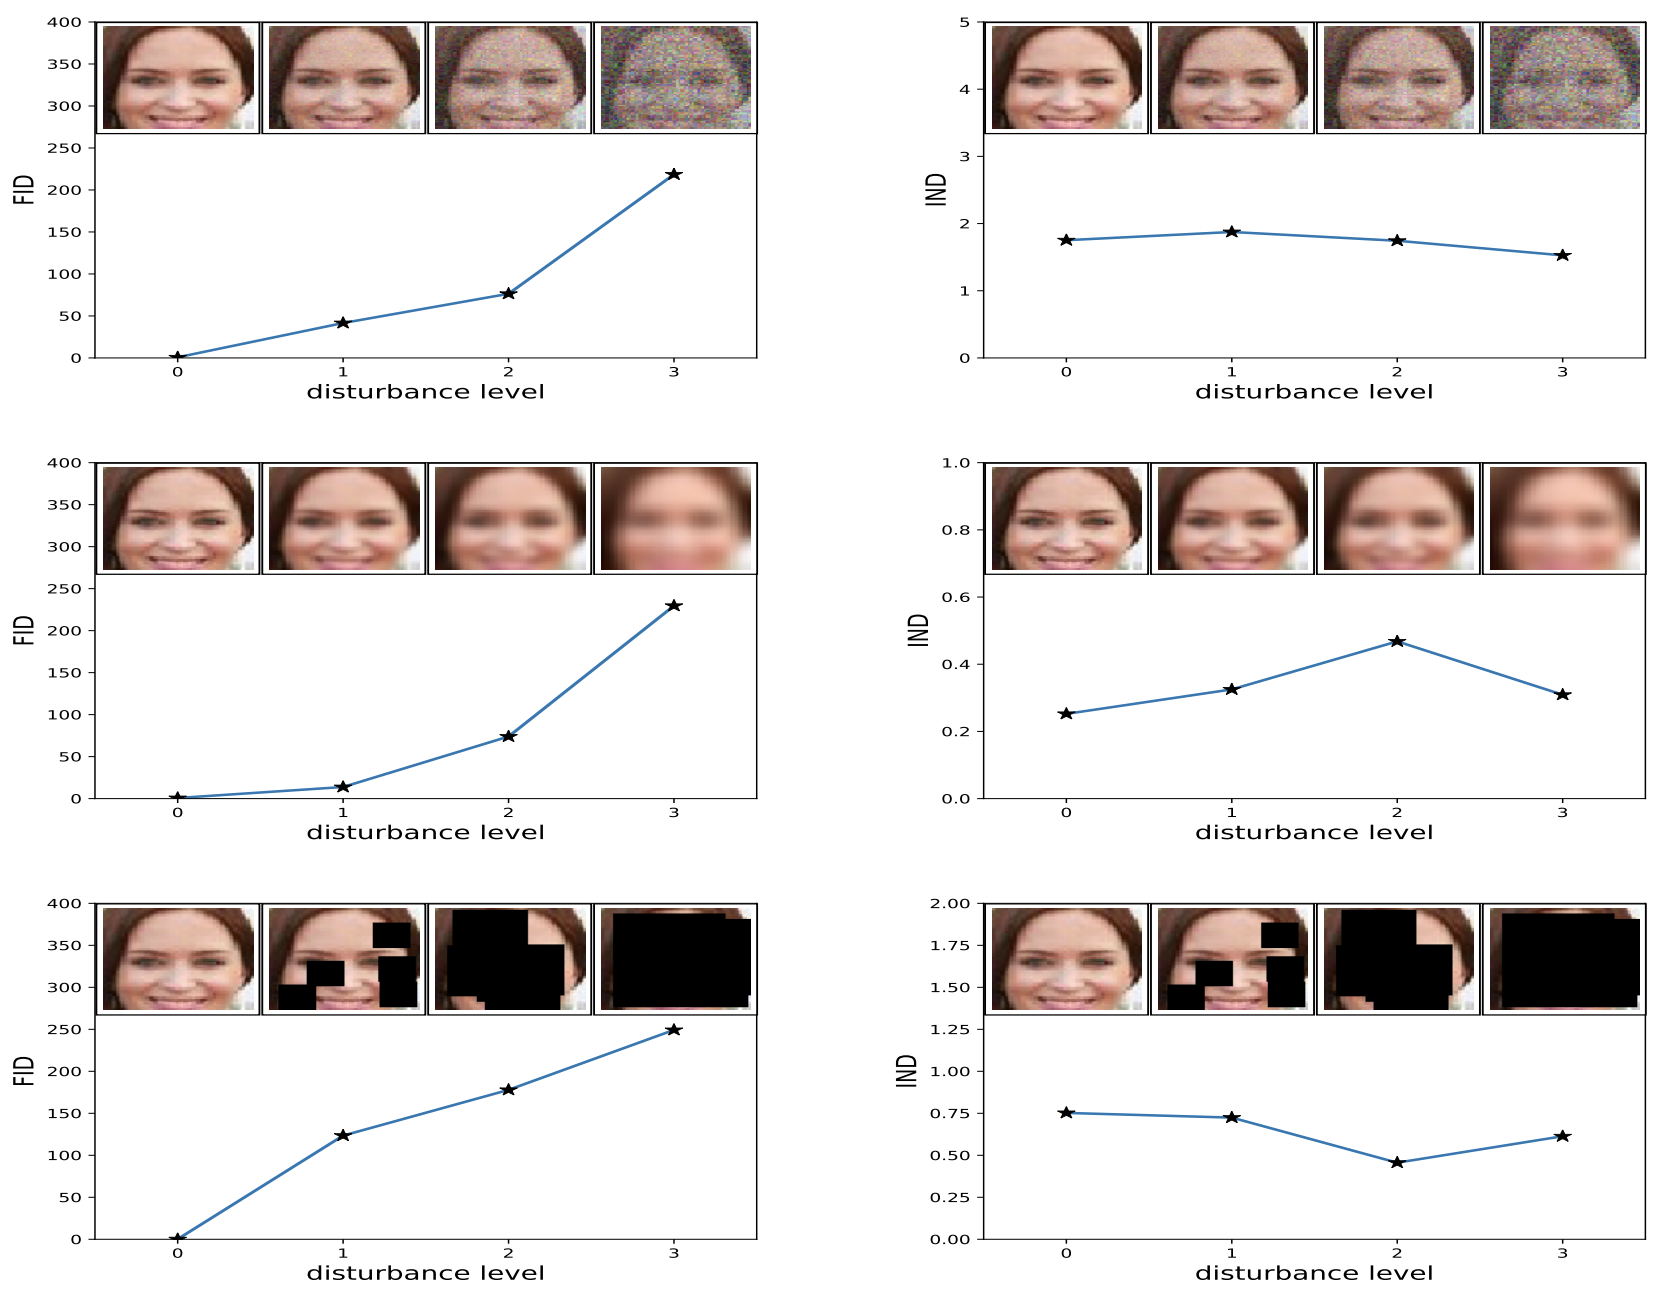
\includegraphics[width=0.9\linewidth]{figs/fid_results}
	\end{figure}
	\vfill
	\hrule\medskip 
	{\scriptsize \href{https://arxiv.org/abs/1706.08500}{https://arxiv.org/abs/1706.08500}}
\end{frame}
%=======
\begin{frame}{Evaluation of likelihood-free models}
	\begin{block}{Frechet Inception Distance}
		\vspace{-0.1cm}
		\[
		D^2 (\pi, p) = \| \mathbf{m}_{\pi} - \mathbf{m}_{p}\|_2^2 + \text{Tr} \left( \bC_{\pi} + \bC_p - 2 \sqrt{\bC_{\pi} \bC_p} \right)
		\]
	\end{block}
	\begin{block}{FID limitations}
		\begin{itemize}
			\item FID depends on the pretrained classification model.
			\item FID needs a large samples  size for evaluation.
			\item Calculation of FID is slow.
			\item FID extimates only two sample moments.
		\end{itemize}
	\end{block}
	\vspace{2cm}

	\vfill
	\hrule\medskip 
	{\scriptsize \href{https://arxiv.org/abs/1706.08500}{https://arxiv.org/abs/1706.08500}}
\end{frame}
%=======
\begin{frame}{Summary}
	\begin{itemize}
		\item Wasserstein GAN uses Kantorovich-Rubinstein duality to estimate Wasserstein distance.
		\item Gradient Penalty proposes the regularizer to enforce Lipschitzness.
		\item Spectral normalization is a weight normalization technique to enforce Lipshitzness.
		\item f-divergence family is a unified framework for divergence minimization.
		\item Inception Score and Frechet Inception Distance are the common metrics for GAN evaluation.
	\end{itemize}
\end{frame}
%=======
\begin{frame}{References}
{\tiny
\begin{itemize}
	
	\item A Note on the Inception Score \\
	\href{https://arxiv.org/abs/1801.01973}{https://arxiv.org/abs/1801.01973} \\
	\textbf{Summary:} Inception Score is not an ideal metric.
	
	\item GANs Trained by a Two Time-Scale Update Rule Converge to a Local Nash Equilibrium \\
	\href{https://arxiv.org/abs/1706.08500}{https://arxiv.org/abs/1706.08500} \\
	\textbf{Summary:} Frechet inception distance was proposed for GAN evaluation.
\end{itemize}
}
\end{frame}
%=======
\end{document} 